\begin{landscape}
\begingroup
\fontsize{10}{13}\selectfont
\fancyhead[L]{\small NACHLASS UND BRIEFWECHSEL}
\renewcommand{\headrulewidth}{0pt}
\par\medskip
\pdfbookmark[2]{Nachlass VII [3]}{pallas-VII-letters3}
\begin{center}[3.]\par\medskip
\textsc{Gauss} an \textsc{Encke}, Göttingen, 7. November 1816.
\end{center}
\par\noindent\hspace*{\parindent}Ihrem gefälligen Anerbieten zu Folge .\ .\ .\ .\ .\ übersende ich Ihnen hier
heute einige Rechnungen für die Pallasstörungen. Zur Erläuterung bemerke
ich zuerst, was noch zu thun ist. Es sind dreierlei Operationen:
\par\noindent\hspace*{\parindent}\textls[100]{Erste Operation} ist bereits ganz abgethan, und ist es daher überflüssig
sie hier näher zu beschreiben.
\par\noindent\hspace*{\parindent}\textls[100]{Zweite Operation} nenne ich die Berechnung von 24 Werthen einer
Function von der Form
\[
\odot)\qquad
\begin{aligned}
&a+a'\cos x+a''\cos2x+a'''\cos3x+\text{etc.}+a^{\mathrm{XII}}\cos12x\\
&\quad+b'\sin x+b''\sin2x+b'''\sin3x+\text{etc.}+b^{\mathrm{XII}}\sin12x
\end{aligned}
\]
\noindent für \(x=0^0\), \(x=15^0\), \(x=30^0\) etc. bis \(x=345^0\). Diese Operation müsste in
allem 126mal gemacht werden, wovon jetzt noch 62 fehlen.
\par\noindent\hspace*{\parindent}\textls[100]{Dritte Operation} nenne ich die 24malige Bestimmung von \(\log r\) und \(\varphi\) aus
\[
\begin{aligned}
r\cos\varphi&=P\\
r\sin\varphi&=Q
\end{aligned}
\]
\SourceLeaf{575}
\noindent wo \(P\) und \(Q\) gegebene (und zwar jede aus der Form \(\odot\) berechnete) Grössen
sind. Diese Operation war in allem 60mal zu machen. Es fehlen jetzt noch 48.
\par\noindent\hspace*{\parindent}Heute schicke ich Ihnen auf 8 Blättchen die Data um 8mal die dritte
Operation zu machen. Jedes \(P\) ergibt sich aus den unten stehenden Zahlen
der Seite, worüber \(\sin A\) steht; jedes \(Q\) aus den Zahlen der andern Seite,
wo \(\cos A\) steht und zwar auf folgende Art. Jedes \(P\) besteht aus zwei Theilen
(die respective aus den cosinus- und sinus-Gliedern entsprungen sind). Diese
zwei Theile finden Sie angegeben und zwar unmittelbar für 13 Werthe in
dieser Ordnung
\providecommand{\VIIthreeStars}[1]{\begin{array}{@{}c@{}}\ast\\\ast\end{array}\;#1}
\begingroup\small
\[
\begin{aligned}
&\begin{array}{c|c|c|c|c|c|c}
\VIIthreeStars{0^0}&\VIIthreeStars{30^0}&\VIIthreeStars{60^0}&\VIIthreeStars{90^0}&\VIIthreeStars{120^0}&\VIIthreeStars{150^0}&\VIIthreeStars{180^0}
\end{array}\\[1ex]
&\begin{array}{c|c|c|c|c|c|}
\VIIthreeStars{15^0}&\VIIthreeStars{45^0}&\VIIthreeStars{75^0}&\VIIthreeStars{105^0}&\VIIthreeStars{135^0}&\VIIthreeStars{165^0}
\end{array}
\end{aligned}
\]
\endgroup
\par\noindent\hspace*{\parindent}Nachher gehts in derselben Ordnung rückwärts, indem immer der zweite
(Sinus-)Theil mit entgegengesetztem Zeichen genommen wird. So ist also z. B.
auf dem ersten Blatt für
\[
\begin{array}{r|r|r}
x&P&Q\\
0^0&+39{,}5723&-24{,}3180\\
15^0&+18{,}4497&-17{,}9717\\
30^0&-1{,}5499&-18{,}3889\\
\vdots&\vdots&\vdots\\
180^0&-6{,}8889&-39{,}1004\\
195^0&-5{,}3849&-40{,}6708\\
210^0&-2{,}6665&-42{,}6184\\
\vdots&\vdots&\vdots
\end{array}
\]
\par\noindent Eine ganze Rechnung der zweiten Operation mache ich auf Einer Octavseite
in dieser Form für
\begingroup\renewcommand{\arraystretch}{1.8}\setlength{\tabcolsep}{13pt}
\begin{center}
\begin{tabular}{|c|c|c|c|c|c|}
\hline
\(0^0\)&\(15^0\)&\(30^0\)&\(45^0\)&\(60^0\)&\(75^0\)\\\hline
\(90^0\)&\(105^0\)&etc.&&&\\\hline
\rule{0pt}{1.8em}&&&&&\\\hline
\rule{0pt}{1.8em}&&&&&\\\hline
\end{tabular}
\end{center}\endgroup
\SourceLeaf{576}
\par\noindent Das erste Carré würde so wie ich die Rechnung mache so aussehen:
\begin{center}
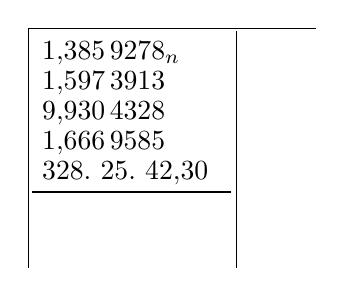
\begin{tikzpicture}[x=1cm,y=1cm]
\draw (0,-.75)--(0,2.30)--(3.65,2.30);
\draw (2.65,-.75)--(2.65,2.27);
\draw (.05,.22)--(2.58,.22);
\node[anchor=west,inner sep=0pt] at (.17,1.98) {\(1{,}385\,9278_n\)};
\node[anchor=west,inner sep=0pt] at (.17,1.60) {\(1{,}597\,3913\)};
\node[anchor=west,inner sep=0pt] at (.17,1.22) {\(9{,}930\,4328\)};
\node[anchor=west,inner sep=0pt] at (.17,.84) {\(1{,}666\,9585\)};
\node[anchor=west,inner sep=0pt] at (.17,.46) {\(328.\ 25.\ 42{,}30\)};
\end{tikzpicture}
\end{center}
\par\noindent Ich lasse nemlich \(\log\operatorname{tang}\varphi\) weg. Ist Ihnen dies
nicht bequem, so schreiben Sie es mit hin.
Dieses ganze Detail bitte ich mir dann aus, zur
bequemern Vergleichung, wenn sich irgendwo
Unterschiede zeigen sollten. Dagegen haben Sie
nicht nöthig, mit gar zu ängstlicher Aufmerksamkeit zu rechnen. Die Ihnen gegenwärtig aufgegebenen Rechnungen werden also 4 Octavblätter füllen; ich sehe es nemlich gern, wenn Sie beide Seiten des Papiers benutzen, um nicht gar zu viel
Papiere zu hüten zu haben. — Ich habe übrigens alle Rechnungen mit 7 Decimalen geführt.
\par\noindent\hspace*{\parindent}Die Ihnen hier gesandten 8 Blätter enthalten zugleich vollständig 16 Ausführungen der zweiten Operation in der Form wie ich sie führe. Um sich
darin zu orientiren, wird die aufmerksame Analyse eines solchen Formulars
besser sein als weitläuftige Vorschriften. Ich bemerke nur, dass immer die
obere Hälfte jedes Blattes die Rechnungen für die Cosinustheile enthält, die
untere die für die Sinustheile. Um Ihnen die Entzifferung zu erleichtern,
mag die Seite .\ .\ .\ .\ .\ als Beispiel dienen. Die Formel \(\odot\) war
\[
\begin{array}{r@{\;}l@{\qquad}r@{\;}l}
+82{,}2072&&&\\
-4{,}7425&\cos x&-13{,}7875&\sin x\\
-2{,}6435&\cos2x&-7{,}5676&\sin2x\\
-0{,}6305&\cos3x&-3{,}8103&\sin3x\\
+0{,}9201&\cos4x&-1{,}9322&\sin4x\\
+1{,}5425&\cos5x&-0{,}5853&\sin5x\\
+0{,}8559&\cos6x&-0{,}2174&\sin6x\\
+0{,}4068&\cos7x&-0{,}0161&\sin7x\\
+0{,}1649&\cos8x&+0{,}0436&\sin8x\\
\multicolumn{2}{c}{0}&\multicolumn{2}{c}{0}\\
\multicolumn{2}{c}{0}&\multicolumn{2}{c}{0}\\
\multicolumn{2}{c}{0}&\multicolumn{2}{c}{0}\\
\multicolumn{2}{c}{0}&\multicolumn{2}{c}{0}
\end{array}
\]
\SourceLeaf{577}
\begin{center}\small
\begin{tabular}{c|c}
\shortstack{Die öfters vorkommenden Zahlen}&\shortstack{sind constante Logarithmen von}\\[.6ex]
\(9{,}787\,0156\)&\(\BareRoot{\frac38}\)\\[.5ex]
\(9{,}849\,4850\)&\(\BareRoot{\frac12}\)\\[.5ex]
\(9{,}937\,5306\)&\(\BareRoot{\frac34}\)
\end{tabular}
\end{center}
\par\noindent Für die zwei Theile der Operation, die mit
\tikz[baseline=-.1em,x=1em,y=1em]{\draw (0,0) rectangle (.72,.72);}
\tikz[baseline=-.1em,x=1em,y=1em]{\draw (0,0) rectangle (.72,.72);\draw (.07,.07) rectangle (.65,.65);}
bezeichnet sind, habe ich
immer dieses Formular bei mir liegen:
\begin{center}
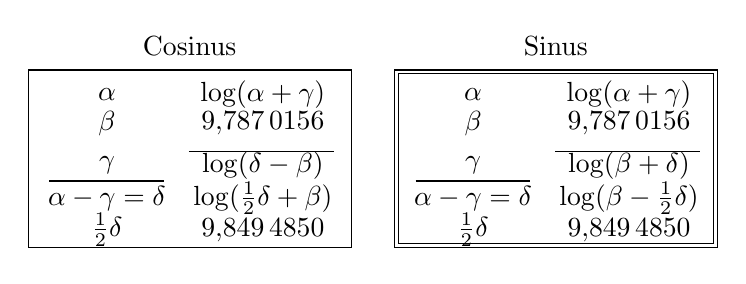
\begin{tikzpicture}[x=1cm,y=1cm]
\node at (2.05,2.55) {Cosinus};
\node at (6.70,2.55) {Sinus};
\draw (0,0) rectangle (4.10,2.25);
\draw (4.65,0) rectangle (8.75,2.25);
\draw (4.70,.05) rectangle (8.70,2.20);
\draw (.27,.84)--(1.72,.84);
\draw (2.04,1.22)--(3.88,1.22);
\draw (4.92,.84)--(6.37,.84);
\draw (6.69,1.22)--(8.53,1.22);
\node at (1.00,1.94) {\(\alpha\)};
\node at (1.00,1.57) {\(\beta\)};
\node at (1.00,1.04) {\(\gamma\)};
\node at (1.00,.62) {\(\alpha-\gamma=\delta\)};
\node at (1.00,.22) {\(\frac12\delta\)};
\node at (2.98,1.94) {\(\log(\alpha+\gamma)\)};
\node at (2.98,1.57) {\(9{,}787\,0156\)};
\node at (2.98,1.04) {\(\log(\delta-\beta)\)};
\node at (2.98,.62) {\(\log(\frac12\delta+\beta)\)};
\node at (2.98,.22) {\(9{,}849\,4850\)};
\node at (5.65,1.94) {\(\alpha\)};
\node at (5.65,1.57) {\(\beta\)};
\node at (5.65,1.04) {\(\gamma\)};
\node at (5.65,.62) {\(\alpha-\gamma=\delta\)};
\node at (5.65,.22) {\(\frac12\delta\)};
\node at (7.63,1.94) {\(\log(\alpha+\gamma)\)};
\node at (7.63,1.57) {\(9{,}787\,0156\)};
\node at (7.63,1.04) {\(\log(\beta+\delta)\)};
\node at (7.63,.62) {\(\log(\beta-\frac12\delta)\)};
\node at (7.63,.22) {\(9{,}849\,4850\)};
\end{tikzpicture}
\end{center}
\par\noindent Das übrige lernt man leicht auswendig.
\par\noindent\hspace*{\parindent}Haben Sie alles herausgebracht, so machen Sie doch einstweilen folgende
zwei Anwendungen: .\ .\ .\ .\ .
\par\medskip
\begin{center}\textsc{Gauss} an \textsc{Encke}, Göttingen, 3. März 1817.\end{center}
\par\noindent\hspace*{\parindent}.\ .\ .\ .\ .\ Vier Elemente, Länge des Perihel, Excentricitätswinkel, Neigung
der Bahn und Länge des Knoten sind nunmehro ganz abgemacht und eingetragen. Was an dem 5. Elemente, der Epoche der Länge, noch zu thun
ist, habe ich mir selbst vorbehalten. Aber bei dem 6., dem Logarithmen
der halben Axe, bin ich so frei Ihre Hülfe nochmals in Anspruch zu nehmen.
\par\noindent .\ .\ .\ .\ .
\clearpage
\endgroup
\end{landscape}
